%!TEX root = ../vernier.tex
\section{Hierarchical Data} \label{sec:hierarchy}
When thinking about a software project, it is very natural to think of it in a hierarchical manner. This hierarchy tends not only to refer to the organization and architecture of a project, but also to the function and behavior of specific entities.

As we mentioned on Section \ref{research_goal}, one of our objectives is to represent the hierarchical relationship in the data. There are many traditional techniques that portray this sort of relationship, each of those with its pros and cons. A few honorable mentions are Squarified and Voronoi Treemaps, Icicle Trees, Sunburst Diagrams, and Circle Packing.
% TODO: add citations

In this application, we have implemented both Squarified Treemap and Sunburst Diagram, each with a different task in mind. Squarified Treemaps are better at using "real state", while Sunsburst Diagrams give a intuitive and unambiguous representation of deep level hierarchies.

\subsection{Squarified Treemap}
A Treemap is a method to display hierarchical data traditionally using a collection of nested rectangles. On this particular project, the nesting of rectangles depicts the package/class hierarchy on the project. The area of each rectangle is defined by the maximum number of lines of code each class has had during the project's history. The area of a package frame is defined by the sum of all classes' areas belonging to it or to it's children packages.

There are several tiling algorithms in the literature with different characteristics (e.g. Ordered Treemaps \cite{ref:orderedtreemap}, Slice and Dice Treemaps\cite{ref:orderedtreemap}, Quantum Treemaps\cite{ref:quantumtreemap}). In addition, several algorithms have been proposed that use non-rectangular regions  \cite{ref:tree1,ref:tree2,ref:tree3}.

But all these techniques offer a trade-off between maintaining the input order and keeping a low aspect-ratio. In our project, the algorithm used to plot these maps is called Squarified Treemaps\cite{ref:squarified}. It prioritizes low aspect-ratios over ordering, reducing the amount of thin, elongated rectangles (see images \ref{fig:comp_treemap1} and \ref{fig:comp_treemap2} ). The results generated by our tool on two Open Source projects can be found on Figures \ref{fig:exo_tree} and \ref{fig:guice_tree}.

\begin{figure}[!tbp]
  \begin{subfigure}[b]{0.4\textwidth}
    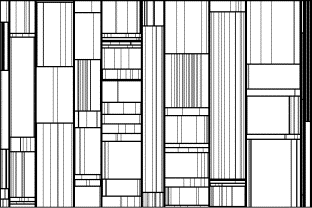
\includegraphics[width=\textwidth]{figures/comp_treemap1.png}
    \caption{Stock portfolio with traditional slice-and-dice layout.}
    \label{fig:comp_treemap1}
  \end{subfigure}
  \hfill
  \begin{subfigure}[b]{0.4\textwidth}
    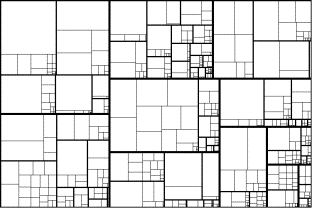
\includegraphics[width=\textwidth]{figures/comp_treemap2.png}
    \caption{Stock portfolio with squarified layout.}
    \label{fig:comp_treemap2}
  \end{subfigure}
  \caption{Treemap layout comparison.}
  \legend{Source: \cite{ref:orderedtreemap}}
\end{figure}

\begin{figure}[H]
  \centering
  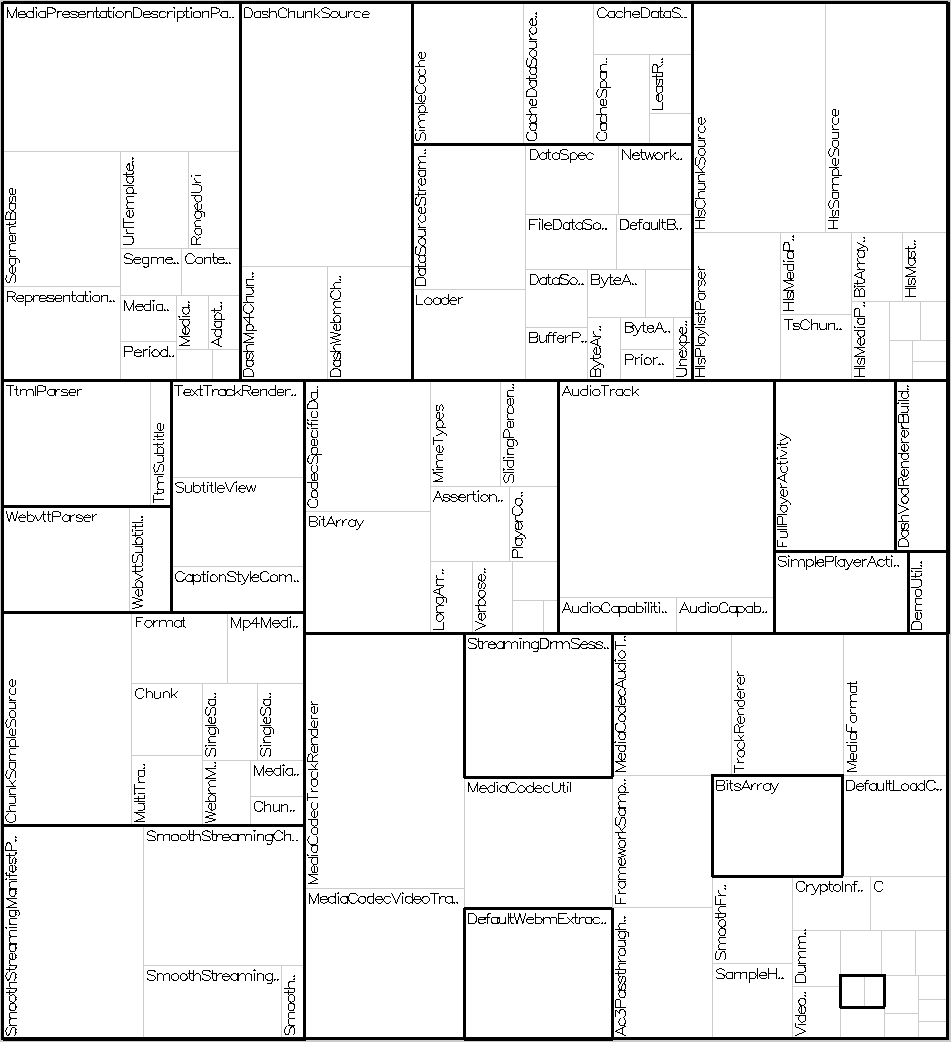
\includegraphics[width=1\textwidth]{figures/exo_tree.png}
  \caption{Google ExoPlayer 117 classes treemap}
  \label{fig:exo_tree}
\end{figure}

\begin{figure}[H]
  \centering
  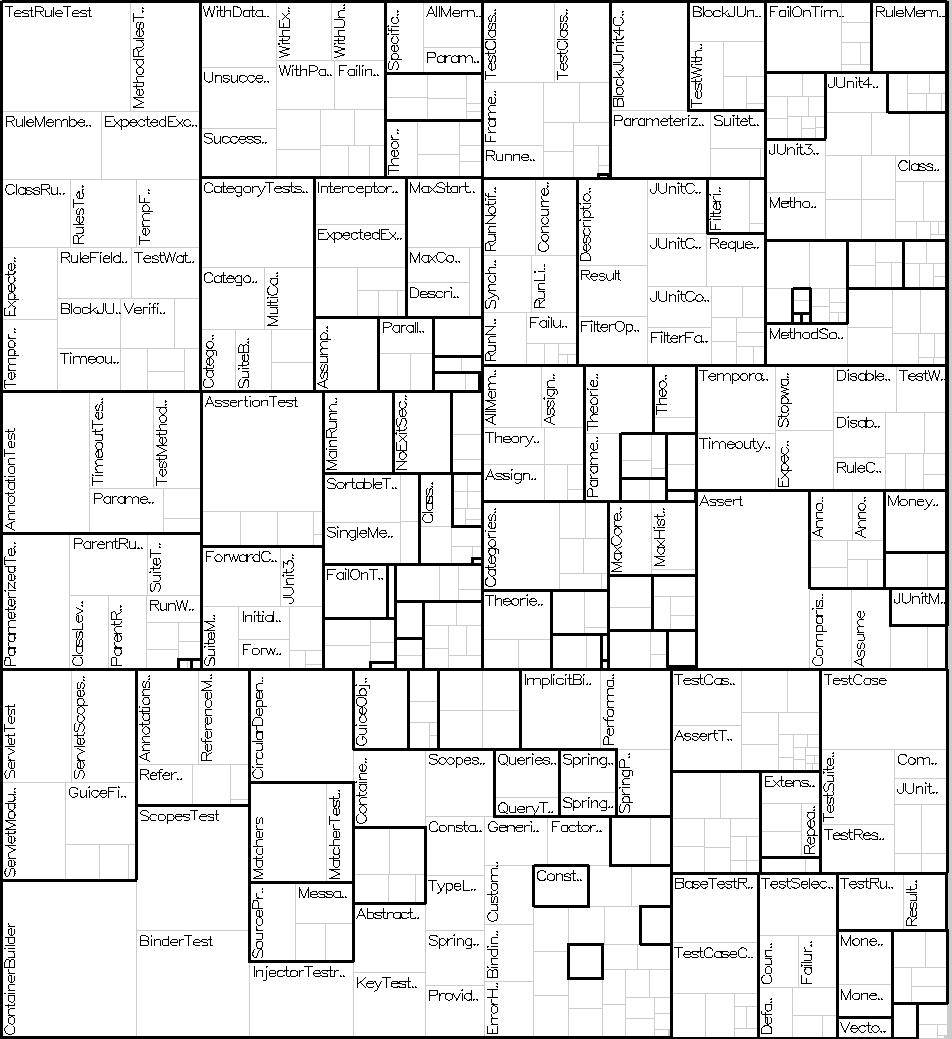
\includegraphics[width=1\textwidth]{figures/guice_tree.png}
  \caption{Google Guice 529 classes treemap}
  \label{fig:guice_tree}
\end{figure}

Squarified treemaps are inherently static, and in order to add information about the dynamic LOC metric value without rearranging the layout, we have encoded in the filled rectangle area the current metric value. The increasing/decreasing of value is shown with a smooth transition between states.

\begin{figure}[H]
  \centering
  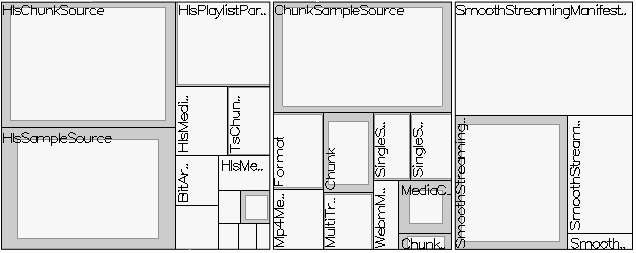
\includegraphics[width=1\textwidth]{figures/dynamic_treemap.png}
  \caption{Base rectangle area represents maximum LOC value and filled rectangle area encode current's}
  \label{fig:dynamic_treemap}
\end{figure}

\subsection{Sunburst Diagram}
This visualization technique uses a series of sliced rings in order to show hierarchy. Each ring corresponds to a level in the hierarchy, with the central circle representing the root node and the hierarchy moving outwards from it.

Rings are sliced up and divided based on their hierarchical relationship to the parent slice. In our project, the angle of each slice is given based on the number of leaf children each node has.

\begin{figure}[H]
  \centering
  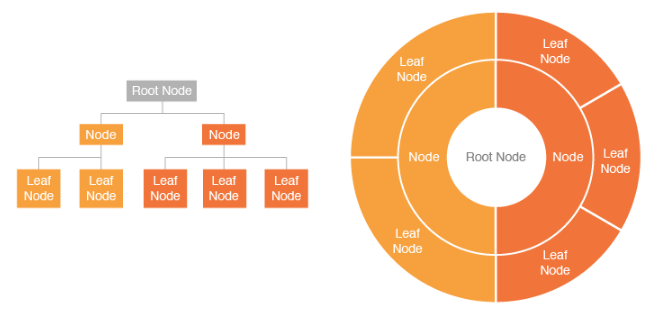
\includegraphics[width=1\textwidth]{figures/sunburst_catalog.png}
  \caption{Representation of hierarchy using Sunburst Diagram}
  \label{fig:sunburst_catalog}
  \legend{Source: \cite{ref:dataviscatalog}}
\end{figure}

\begin{figure}[H]
  \centering
  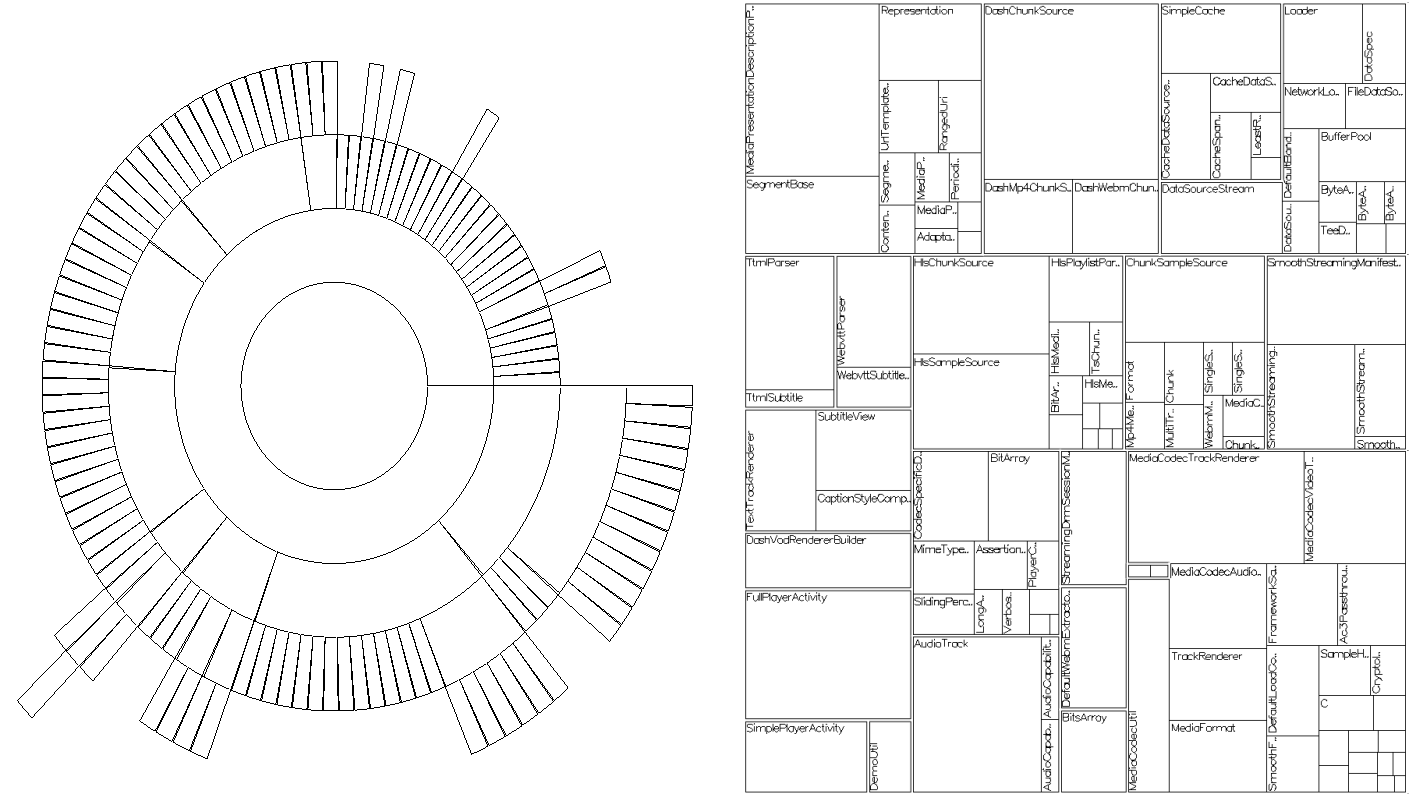
\includegraphics[width=1\textwidth]{figures/sun_tree_comp.png}
  \caption{Representation of the ExoPlayer's project hierarchy using both Sunburst Diagram and Squarified Treeemap}
  \label{fig:sun_tree_comp}
\end{figure}
